\documentclass[journal, a4paper]{IEEEtran}

% some very useful LaTeX packages include:

\usepackage{biblatex}
\addbibresource{cite.bib}


%\usepackage{cite}      % Written by Donald Arseneau
                        % V1.6 and later of IEEEtran pre-defines the format
                        % of the cite.sty package \cite{} output to follow
                        % that of IEEE. Loading the cite package will
                        % result in citation numbers being automatically
                        % sorted and properly "ranged". i.e.,
                        % [1], [9], [2], [7], [5], [6]
                        % (without using cite.sty)
                        % will become:
                        % [1], [2], [5]--[7], [9] (using cite.sty)
                        % cite.sty's \cite will automatically add leading
                        % space, if needed. Use cite.sty's noadjust option
                        % (cite.sty V3.8 and later) if you want to turn this
                        % off. cite.sty is already installed on most LaTeX
                        % systems. The latest version can be obtained at:
                        % http://www.ctan.org/tex-archive/macros/latex/contrib/supported/cite/

\usepackage{graphicx}   % Written by David Carlisle and Sebastian Rahtz
                        % Required if you want graphics, photos, etc.
                        % graphicx.sty is already installed on most LaTeX
                        % systems. The latest version and documentation can
                        % be obtained at:
                        % http://www.ctan.org/tex-archive/macros/latex/required/graphics/
                        % Another good source of documentation is "Using
                        % Imported Graphics in LaTeX2e" by Keith Reckdahl
                        % which can be found as esplatex.ps and epslatex.pdf
                        % at: http://www.ctan.org/tex-archive/info/

%\usepackage{psfrag}    % Written by Craig Barratt, Michael C. Grant,
                        % and David Carlisle
                        % This package allows you to substitute LaTeX
                        % commands for text in imported EPS graphic files.
                        % In this way, LaTeX symbols can be placed into
                        % graphics that have been generated by other
                        % applications. You must use latex->dvips->ps2pdf
                        % workflow (not direct pdf output from pdflatex) if
                        % you wish to use this capability because it works
                        % via some PostScript tricks. Alternatively, the
                        % graphics could be processed as separate files via
                        % psfrag and dvips, then converted to PDF for
                        % inclusion in the main file which uses pdflatex.
                        % Docs are in "The PSfrag System" by Michael C. Grant
                        % and David Carlisle. There is also some information
                        % about using psfrag in "Using Imported Graphics in
                        % LaTeX2e" by Keith Reckdahl which documents the
                        % graphicx package (see above). The psfrag package
                        % and documentation can be obtained at:
                        % http://www.ctan.org/tex-archive/macros/latex/contrib/supported/psfrag/

%\usepackage{subfigure} % Written by Steven Douglas Cochran
                        % This package makes it easy to put subfigures
                        % in your figures. i.e., "figure 1a and 1b"
                        % Docs are in "Using Imported Graphics in LaTeX2e"
                        % by Keith Reckdahl which also documents the graphicx
                        % package (see above). subfigure.sty is already
                        % installed on most LaTeX systems. The latest version
                        % and documentation can be obtained at:
                        % http://www.ctan.org/tex-archive/macros/latex/contrib/supported/subfigure/

\usepackage{url}        % Written by Donald Arseneau
                        % Provides better support for handling and breaking
                        % URLs. url.sty is already installed on most LaTeX
                        % systems. The latest version can be obtained at:
                        % http://www.ctan.org/tex-archive/macros/latex/contrib/other/misc/
                        % Read the url.sty source comments for usage information.

%\usepackage{stfloats}  % Written by Sigitas Tolusis
                        % Gives LaTeX2e the ability to do double column
                        % floats at the bottom of the page as well as the top.
                        % (e.g., "\begin{figure*}[!b]" is not normally
                        % possible in LaTeX2e). This is an invasive package
                        % which rewrites many portions of the LaTeX2e output
                        % routines. It may not work with other packages that
                        % modify the LaTeX2e output routine and/or with other
                        % versions of LaTeX. The latest version and
                        % documentation can be obtained at:
                        % http://www.ctan.org/tex-archive/macros/latex/contrib/supported/sttools/
                        % Documentation is contained in the stfloats.sty
                        % comments as well as in the presfull.pdf file.
                        % Do not use the stfloats baselinefloat ability as
                        % IEEE does not allow \baselineskip to stretch.
                        % Authors submitting work to the IEEE should note
                        % that IEEE rarely uses double column equations and
                        % that authors should try to avoid such use.
                        % Do not be tempted to use the cuted.sty or
                        % midfloat.sty package (by the same author) as IEEE
                        % does not format its papers in such ways.

\usepackage{amsmath}    % From the American Mathematical Society
                        % A popular package that provides many helpful commands
                        % for dealing with mathematics. Note that the AMSmath
                        % package sets \interdisplaylinepenalty to 10000 thus
                        % preventing page breaks from occurring within multiline
                        % equations. Use:
%\interdisplaylinepenalty=2500
                        % after loading amsmath to restore such page breaks
                        % as IEEEtran.cls normally does. amsmath.sty is already
                        % installed on most LaTeX systems. The latest version
                        % and documentation can be obtained at:
                        % http://www.ctan.org/tex-archive/macros/latex/required/amslatex/math/



% Other popular packages for formatting tables and equations include:

%\usepackage{array}
% Frank Mittelbach's and David Carlisle's array.sty which improves the
% LaTeX2e array and tabular environments to provide better appearances and
% additional user controls. array.sty is already installed on most systems.
% The latest version and documentation can be obtained at:
% http://www.ctan.org/tex-archive/macros/latex/required/tools/

% V1.6 of IEEEtran contains the IEEEeqnarray family of commands that can
% be used to generate multiline equations as well as matrices, tables, etc.

% Also of notable interest:
% Scott Pakin's eqparbox package for creating (automatically sized) equal
% width boxes. Available:
% http://www.ctan.org/tex-archive/macros/latex/contrib/supported/eqparbox/

% *** Do not adjust lengths that control margins, column widths, etc. ***
% *** Do not use packages that alter fonts (such as pslatex).         ***
% There should be no need to do such things with IEEEtran.cls V1.6 and later.


% Your document starts here!
\begin{document}
\begin{titlepage}

\newcommand{\HRule}{\rule{\linewidth}{0.5mm}} % Defines a new command for the horizontal lines, change thickness here

\center % Center everything on the page
 %----------------------------------------------------------------------------------------
%	LOGO SECTION
%----------------------------------------------------------------------------------------

~\\[1cm]

\includegraphics{SCUT.png}\\[2cm] % Include a department/university logo - this will require the graphicx package

%----------------------------------------------------------------------------------------
%	TITLE SECTION
%----------------------------------------------------------------------------------------

\HRule \\[1cm]
{ \huge \bfseries The Experiment I Report of \textit{Machine Learning} }\\[0.6cm] % Title of your document
\HRule \\[2cm]
%----------------------------------------------------------------------------------------
%	HEADING SECTIONS
%----------------------------------------------------------------------------------------


\textsc{\LARGE \textbf{School:} School of Software Engineering}\\[1cm]
\textsc{\LARGE \textbf{Subject:} Software Engineering}\\[2cm] 

 
%----------------------------------------------------------------------------------------
%	AUTHOR SECTION
%----------------------------------------------------------------------------------------

\begin{minipage}{0.4\textwidth}
\begin{flushleft} \large
\emph{Author:}\\
Jianqiao Hu % Your name
\end{flushleft}
\end{minipage}
~
\begin{minipage}{0.4\textwidth}
\begin{flushright} \large
\emph{Supervisor:} \\
Qingyao Wu % Supervisor's Name
\end{flushright}
\end{minipage}\\[2cm]
~
\begin{minipage}{0.4\textwidth}
\begin{flushleft} \large
\emph{Student ID:}\\
202221045886
\end{flushleft}
\end{minipage}
~
\begin{minipage}{0.4\textwidth}
\begin{flushright} \large
\emph{Grade:} \\
Graduate
\end{flushright}
\end{minipage}\\[2cm]

% If you don't want a supervisor, uncomment the two lines below and remove the section above
%\Large \emph{Author:}\\
%John \textsc{Smith}\\[3cm] % Your name

%----------------------------------------------------------------------------------------
%	DATE SECTION
%----------------------------------------------------------------------------------------

{\large \today}\\[2cm] % Date, change the \today to a set date if you want to be precise

 
%----------------------------------------------------------------------------------------

\vfill % Fill the rest of the page with whitespace

\end{titlepage}


% Define document title and author
	\title{Face Detection Based on Neural Network}
	\author{Jianqiao Hu \thanks{autor's email: 202221045886@mail.scut.edu.cn}}
	\maketitle

% Write abstract here
\begin{abstract}
This report is about first experience in machine learning. We explained how to build a anaconda environment to launch python scripts. In second part, three deep learning models to face detection was been used. Consequently, statistics of this experience was been showed and in the final, we have attached some face detection results to reveal utility of models.
\end{abstract}

% Each section begins with a \section{title} command
\section{Introduction}
	% \PARstart{}{} creates a tall first letter for this first paragraph
\PARstart{F}{ace} detection is an important research hotspot in computer vision research field. Nowadays, it plays a significant role in auto-driving and smart home IoT system. Some methods like \cite{ZHAN201619} and \cite{8080244} used convolutional neural network (CNN). This experience use method raised by \cite{7553523} to detection faces in photos.

% Main Part
\section{Methods and Theory}
In \cite{8080244}, it propose Multi-task convolutional neural network to detect faces from images. Our experience used this method to handle photos in dataset. Whole Model includes three sub-models which are Proposal Network(P-Net), Refine Network(R-Net) and Output Network(O-Net). Each of these sub-models has its assignment respectively, in which generating bounding boxes for P-Net, removing no-face bounding boxes for R-Net while add landmark in photos for O-Net.

The learning objective is formulated as a two-class classification problem. For each sample $x_{i}$, this method uses the cross-entropy loss as equation.\ref{loss1}, where $p_{i}$ is the probability produced by the network that indicates a sample being a face.



\begin{equation}
    L_{i}^{det}=-(y_{i}^{det}log(p_{i})+(1-y_{i}^{det})(1-log(p_{i})) )\label{loss1}
\end{equation}

For each candidate window, we  predict the offset between it and the nearest ground truth (i.e., the bounding boxes’ left top, height, and width). The learning objective is formulated as a regression problem, and this method employed the Euclidean loss for each sample $x_{i}$ as equation.\ref{eq2}.
\begin{equation}
    L_{i}^{box}=\Vert \hat{y}_{i}^{box}-y_{i}^{box} \Vert_2^{2} \label{eq2}
\end{equation}

This model's loss in labels can be implemented directly with a sample type indicator. While the overall learning target can be formulated as equation.\ref{target1}.

\begin{equation}
    min\sum\limits_{i=1}^{N}\sum\limits_{j \in \left det,box,landmark \right }\alpha_{j} \beta_{i}^{j} L_{i}^{j}\label{target1}
\end{equation}


\section{Experiments}
\subsection{Dataset}
Training dataset includes more than ten thousand photos and all of them has at least one people facing to camera. Test dataset includes more than one thousand photos. In experience's testing procession, all images in test dataset were been marked by O-Net. Training process cost many time because this experience needs lots GPU processing power. In final, we uesd the parameter file provided with code to verify the model's responsibility in face detection.

\subsection{Result}
We used the parameters archive files provided by Github repository to test truly effect of these three models. Program scripts load images from test photos folder, annotated them by face in and converted annotated images into result folder. Whole test processing cost about 9 sec. by a laptop with a GPU as NVIDIA GTX 950M. Time costing result revealing printscreens are Fig.\ref{fig:cost}.  We picked two of them to explain the effects of face detection, both of them have at least two person in it. First photo like Fig.\ref{fig:13869_raw} includes two persons, while one of them was back to the camera and another was frontal. So only face-to-camera one's face was been annotated by program like Fig.\ref{fig:13869}. Another photo that three person in was been annotated exactly with all the people like Fig.\ref{fig:13692}

	% You can reference tables and figure by using the \ref{label} command. Each table and figure needs to have a UNIQUE label.
% 	Figures and tables should be labeled and numbered, such as in Table~\ref{tab:simParameters} and Fig.~\ref{fig:tf_plot} and \ref{fig:13869}.

	% This is how you define a table: the [!hbt] means that LaTeX is forced (by the !) to place the table exactly here (by h), or if that doesnt work because of a pagebreak or so, it tries to place the table to the bottom of the page (by b) or the top (by t).
% 	\begin{table}[!hbt]
% 		% Center the table
% 		\begin{center}
% 		% Title of the table
% 		\caption{Simulation Parameters}
% 		\label{tab:simParameters}
% 		% Table itself: here we have two columns which are centered and have lines to the left, right and in the middle: |c|c|
% 		\begin{tabular}{|c|c|}
% 			% To create a horizontal line, type \hline
% 			\hline
% 			% To end a column type &
% 			% For a linebreak type \\
% 			Information message length & $k=16000$ bit \\
% 			\hline
% 			Radio segment size & $b=160$ bit \\
% 			\hline
% 			Rate of component codes & $R_{cc}=1/3$\\
% 			\hline
% 			Polynomial of component encoders & $[1 , 33/37 , 25/37]_8$\\
% 			\hline
% 		\end{tabular}
% 		\end{center}
% 	\end{table}

	% If you have questions about how to write mathematical formulas in LaTeX, please read a LaTeX book or the 'Not So Short Introduction to LaTeX': tobi.oetiker.ch/lshort/lshort.pdf

	% This is how you include a eps figure in your document. LaTeX only accepts EPS or TIFF files.
% 	\begin{figure}[!hbt]
% 		% Center the figure.
% 		\begin{center}
% 		% Include the eps file, scale it such that it's width equals the column width. You can also put width=8cm for example...
% 		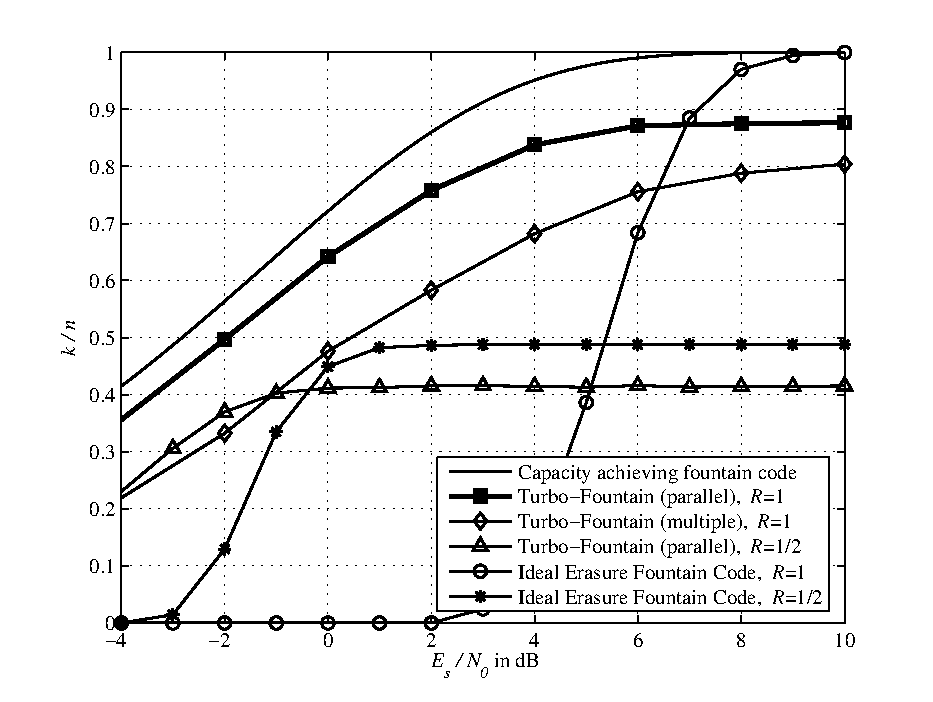
\includegraphics[width=\columnwidth]{plot_tf}
% 		% Create a subtitle for the figure.
% 		\caption{Simulation results on the AWGN channel. Average throughput $k/n$ vs $E_s/N_0$.}
% 		% Define the label of the figure. It's good to use 'fig:title', so you know that the label belongs to a figure.
% 		\label{fig:tf_plot}
% 		\end{center}
% 	\end{figure}
	
		\begin{figure}
		% Center the figure.
		\begin{center}
		% Include the eps file, scale it such that it's width equals the column width. You can also put width=8cm for example...
		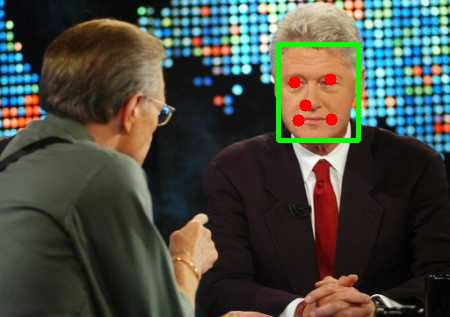
\includegraphics[width=\columnwidth]{images/13869.jpg}
		% Create a subtitle for the figure.
		\caption{result with a person}
		% Define the label of the figure. It's good to use 'fig:title', so you know that the label belongs to a figure.
		\label{fig:13869}
		\end{center}
	\end{figure}
	
	\begin{figure}
		% Center the figure.
		\begin{center}
		% Include the eps file, scale it such that it's width equals the column width. You can also put width=8cm for example...
		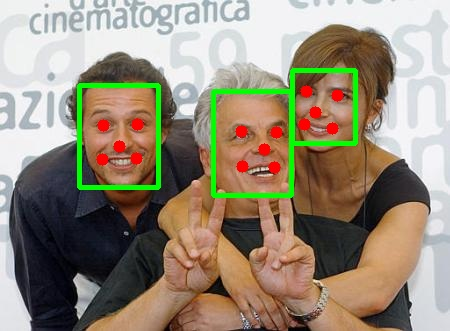
\includegraphics[width=\columnwidth]{images/13692.jpg}
		% Create a subtitle for the figure.
		\caption{result with three person}
		% Define the label of the figure. It's good to use 'fig:title', so you know that the label belongs to a figure.
		\label{fig:13692}
		\end{center}
	\end{figure}
	
	\begin{figure}
		% Center the figure.
		\begin{center}
		% Include the eps file, scale it such that it's width equals the column width. You can also put width=8cm for example...
		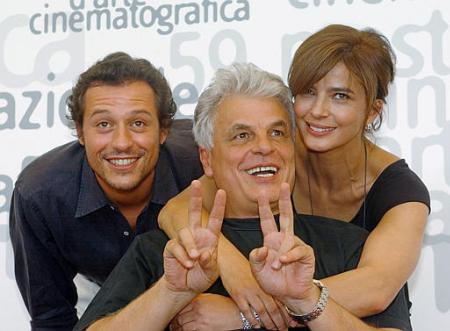
\includegraphics[width=\columnwidth]{images/img_13692.jpg}
		% Create a subtitle for the figure.
		\caption{three person in a photo}
		% Define the label of the figure. It's good to use 'fig:title', so you know that the label belongs to a figure.
		\label{fig:13692_raw}
		\end{center}
	\end{figure}
	
	\begin{figure}
		% Center the figure.
		\begin{center}
		% Include the eps file, scale it such that it's width equals the column width. You can also put width=8cm for example...
		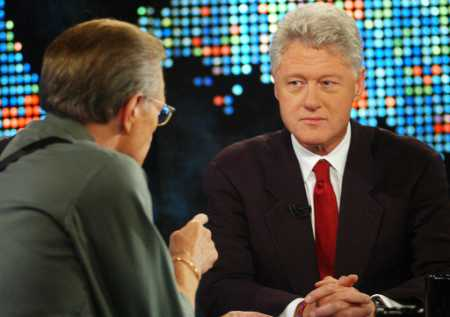
\includegraphics[width=\columnwidth]{images/img_13869.jpg}
		% Create a subtitle for the figure.
		\caption{two person in a photo}
		% Define the label of the figure. It's good to use 'fig:title', so you know that the label belongs to a figure.
		\label{fig:13869_raw}
		\end{center}
	\end{figure}
	\begin{figure}
		% Center the figure.
		\begin{center}
		% Include the eps file, scale it such that it's width equals the column width. You can also put width=8cm for example...
		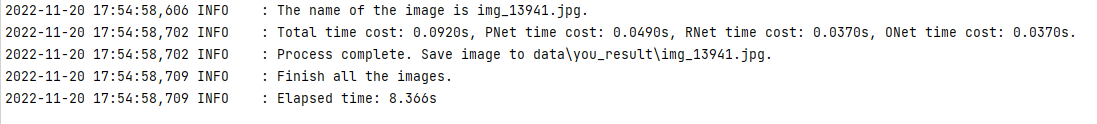
\includegraphics[width=\columnwidth]{images/cost.png}
		% Create a subtitle for the figure.
		\caption{cost time}
		% Define the label of the figure. It's good to use 'fig:title', so you know that the label belongs to a figure.
		\label{fig:cost}
		\end{center}
	\end{figure}

\section{Conclusion}
	Multi-task convolutional neural network can play a crucial role in face detection. In this experience, we use three models to detect faces in photos. Due to lots parameter in models, it cost a long time to train all detection model in laptop. In training processing, we used late version pytorch to train models so python interpreter gave a warning in \textit{torch.nn}. In this experience, we used a machine learning to handle a mission in face detection, it realized me that different networks in model has its responsibilities respectively, in which generating bounding boxes for P-Net, removing no-face bounding boxes for R-Net while add landmark in photos for O-Net.
	
	Training this model to handle face detecting cost many time in a laptop. And this experience's result needs tensorflow library to show the result of images of data. In the final, we conjectured that if P=Net and O-Net could be trained parallelly, it would save many time in training.

\printbibliography

% Your document ends here!
\end{document}

